\documentclass[a4paper]{article}

%% Language and font encodings
\usepackage[english]{babel}
\usepackage[utf8x]{inputenc}

\usepackage{booktabs}
\usepackage{tabu}
\usepackage[T1]{fontenc}

%% Sets page size and margins
\usepackage[a4paper,top=3cm,bottom=2cm,left=3cm,right=3cm,marginparwidth=1.75cm]{geometry}

%% Useful packages
\usepackage{amsmath}
\usepackage{graphicx}
\usepackage{titling}
%\usepackage{apacite}
\usepackage[colorinlistoftodos]{todonotes}
\usepackage[colorlinks=true, allcolors=blue]{hyperref}
\usepackage[strings]{underscore}


\title{Modeling and 3D Printing Sea Shells\\
		\large Final Report}
\author{Edward Ye || 100972832}
\date{2019/04/22}

\begin{document}
\maketitle

\begin{abstract}
	I thought sea shells were cool so I made some models and 3D printed them.
\end{abstract}

\tableofcontents

\section{Some Background and Motivation}

Sea shells have interesting patterns which  appear to be readily described by mathematics and computation. Work has already been done to describe aspects of sea shells, from the spiral shape to the color patterns to the protrusions found on the exterior \cite{Galbraith00modelingmurex}\cite{abss}\cite{VANDERHELM1998505}. Recently some work has also gone into the 3D printing of sea shell model \cite{3dprinting-seashells}\cite{bachman-3dprinting}.

The motivation of this project will be to extend the methods of generating the exterior protrusions to be able to mimic a wider variety of shells. Prusinkiewicz and Fowler have modeled periodic ridge and bump patterns and they have also combined multiple generating curves to imitate more intricate shells \cite{abss}. Galbraith et al. have used constructive solid geometry (CSG) to compose different modules to generate a complete Murex Cabritii model. They have proposed the use of reaction-diffusion (RD) to place protrusions algorithmically \cite{Galbraith00modelingmurex}. Intuitively this appears to be a reasonable idea since the protrusion placement of certain shells are something like the placement of spots upon a leopard. Such patterns have already been described as textures using RD \cite{Turk:1991:GTA:127719.122749}.

\pagebreak

\subsection{Main Objective}

An interesting candidate for such a method would be:

\begin{figure}[h]
	\centering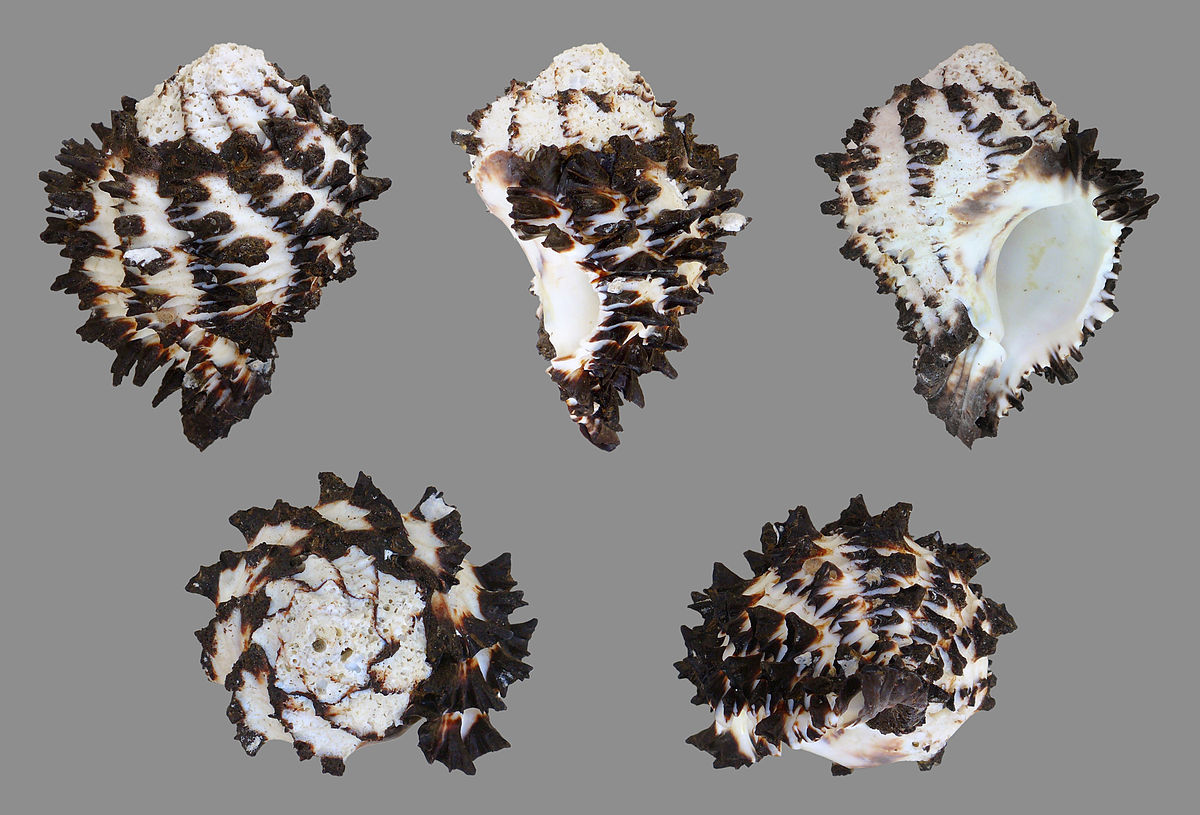
\includegraphics[scale=0.25]{./img/hexaplex_radix.jpg}
	\caption{Hexaplex radix \cite{wikipedia-hexaplex}}
	\label{fig:hexaplex-radix} % Unique label used for referencing the figure in-text
	%\addcontentsline{toc}{figure}{Figure \ref{fig:placeholder}} % Uncomment to add the figure to the table of contents
\end{figure}

The main objective would be to create a model that closely resembles the shell and to 3D print it.

\section{Implicit Surface}

The initial idea was to use a raytracer, such as POV-Ray, to create an implicit surface (isosurface in POV-Ray terminology) that would represent the shell model. The software allows for textures to also act as functions, so that the sum of the implicit equation and the texture function would generate the desired surface. POV-Ray could then generate a point cloud that would form a mesh to be 3-D printed.

\subsection{Logarithmic Spiral}

Shells are modeled by logarithmic spirals. In polar coordinates the logarithmic spiral equation is:

\begin{equation}
	r = Ae^{\alpha \theta}
\end{equation}

Where $A$ shifts the position of the spiral inward or outward, and $\alpha$ multiples the growth rate $(\frac{dr}{d\theta} = \alpha A e^{\alpha \theta} = \alpha r)$.

\begin{figure}[h]
	\centering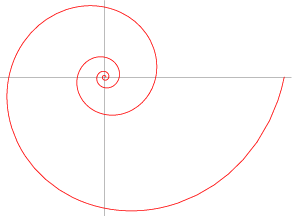
\includegraphics[scale=0.7]{./img/logarithmic-spiral.png}
	\caption{2-D Logarithmic Spiral using equation (1). \cite{logspiral}}
	\label{fig:log-spiral} % Unique label used for referencing the figure in-text
	%\addcontentsline{toc}{figure}{Figure \ref{fig:placeholder}} % Uncomment to add the figure to the table of contents
\end{figure}

\pagebreak

In 3-D Cartesian coordinates (1) can be represented as:

$$ r = \sqrt{x^2 + y^2 + z^2 } $$
$$ \theta = tan^{-1}({\frac{y}{x}}) $$

\begin{equation}
	\sqrt{x^2 + y^2 + z^2 } = A e^{\alpha \cdot tan^{-1}({\frac{y}{x}})}
\end{equation}

Squaring both sides of (2) then gives the implicit equation:

\begin{equation}
	s(x,y,z) = x^2 + y^2 + z^2 - A e^{2 \alpha \cdot tan^{-1}({\frac{y}{x}})} = 0
\end{equation}

\begin{figure}[h]
	\centering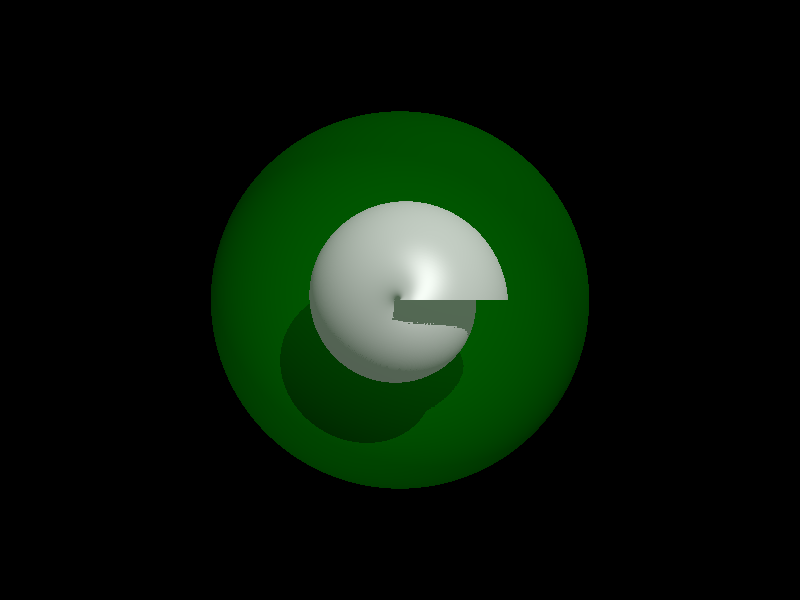
\includegraphics[scale=0.3]{./img/logspiral.png}
	\caption{3-D log spiral generated by \textit{logspiral.pov} using an implementation of equation (3).}
	\label{fig:3d-log-spiral} % Unique label used for referencing the figure in-text
	%\addcontentsline{toc}{figure}{Figure \ref{fig:placeholder}} % Uncomment to add the figure to the table of contents
\end{figure}

If I have some other function, such as $f_{noise}(x,y,z)$, I can add it to equation (3) to get another implicit equation:

\begin{equation}
	s(x,y,z) + f_{noise}(x,y,z) = 0
\end{equation}

\begin{figure}[h]
	\centering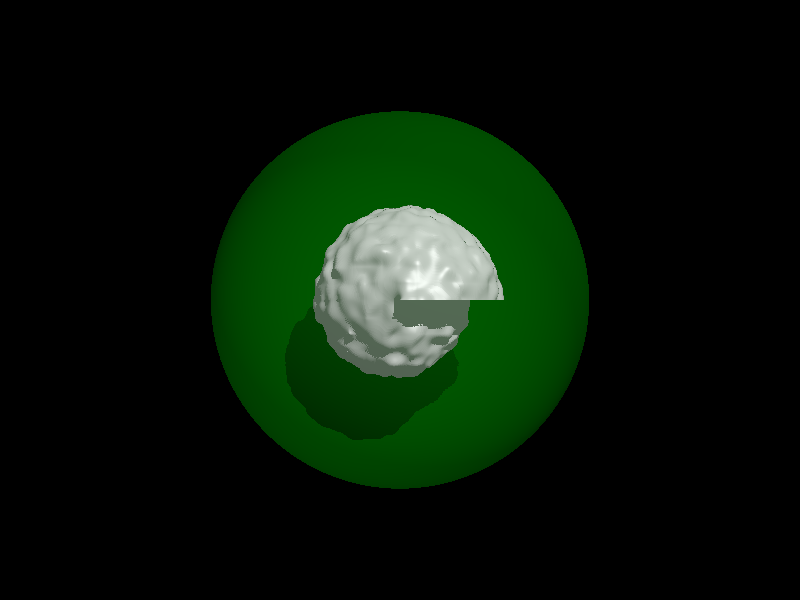
\includegraphics[scale=0.3]{./img/logspiral_noise.png}
	\caption{Equation (4) gives something pretty ugly.}
	\label{fig:3d-log-spiral-noise} % Unique label used for referencing the figure in-text
	%\addcontentsline{toc}{figure}{Figure \ref{fig:placeholder}} % Uncomment to add the figure to the table of contents
\end{figure}

After fiddling around with this for a while it became apparent that the existing parametric equations describing shells could not be easily turned into implicit equations.

\section{Parametric Equations}

Two kinds of parametric equations will be discussed: the first is modified torus used in \cite{povray-seashells}, and the other is a logarithmic spiral with a generating curve used in \cite{JORGEPICADO}.

\subsection{Modified Torus}

The parametric equation for a torus is:

\begin{equation}
	\begin{cases}
		x = (c + a \cdot cos(v)) cos(u)\\
		y = (c + a \cdot cos(v)) sin(u)\\
		z = a \cdot sin(v)\\
	\end{cases}
\end{equation}

for $u,v \in  [0, 2\pi)$.

\begin{figure}[h]
	\centering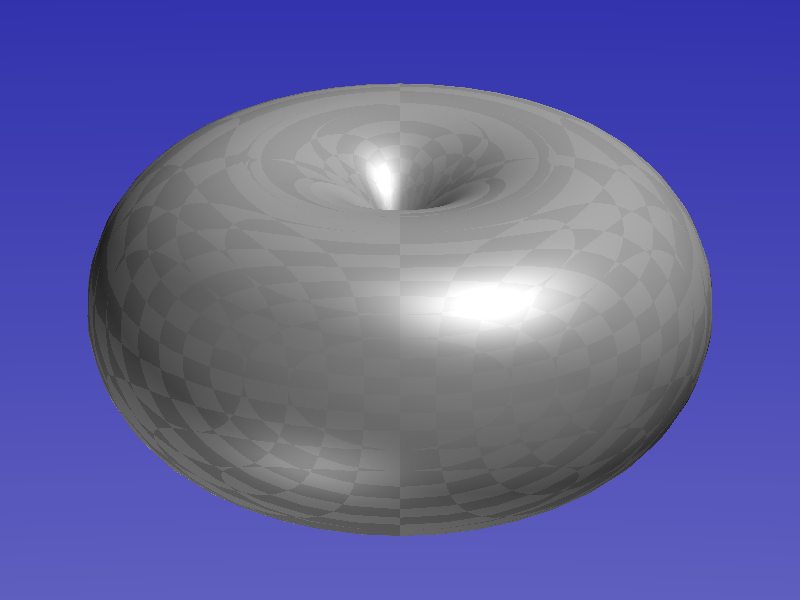
\includegraphics[scale=0.3]{./img/torus.png}
	\caption{Raytraced torus using equation 5.}
	\label{torus} % Unique label used for referencing the figure in-text
	%\addcontentsline{toc}{figure}{Figure \ref{fig:placeholder}} % Uncomment to add the figure to the table of contents
\end{figure}

A simple way to create models resembling sea shells is to form a linear spiral that grows downward as described in \cite{povray-seashells}. The basic equation used is:

\begin{equation}
	\begin{cases}
		w(u) = \frac{u}{2\pi}\\
		x = w(u) \cdot [c + a \cdot cos(v)] cos(N \cdot u)\\
		y = w(u) \cdot [c + a \cdot cos(v)] sin(N \cdot u)\\
		z = w(u) \cdot a \cdot sin(v) + H \cdot [w(u)]^2\\
	\end{cases}
\end{equation}

Where $H$ is the height and $N$ is the number of turns of the spiral. $w(u)$ ensures that the spiral grows linearly from $0$ to $1$, and is used quadratically in the $z$ parameter, so that the height doesn't grow too quickly downward.

\begin{figure}[h]
	\centering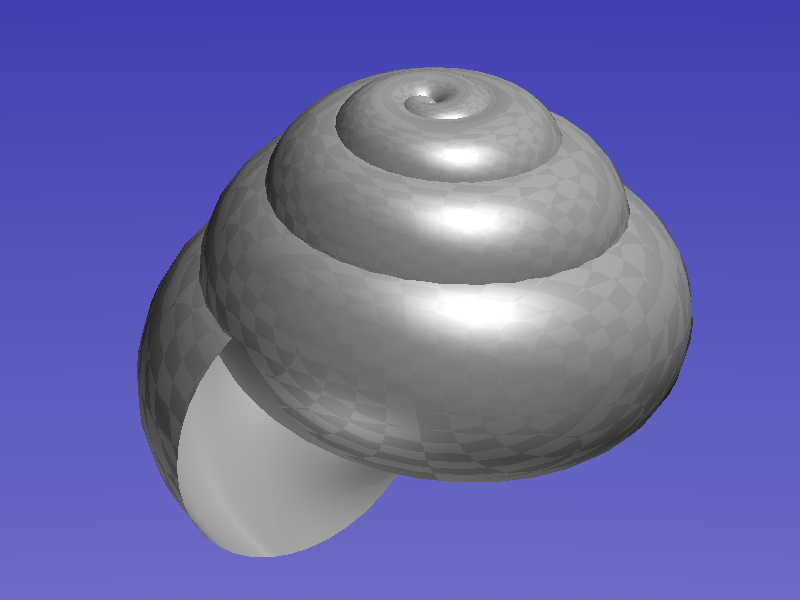
\includegraphics[scale=0.3]{./img/ShellPeriwinkle.png}
	\caption{Periwinkle shell using equation 6, where $a = 1$, $c = 1$, $N = 4.6$ and $H = 2$. \cite{povray-seashells}}
	\label{periwinkle} % Unique label used for referencing the figure in-text
	%\addcontentsline{toc}{figure}{Figure \ref{fig:placeholder}} % Uncomment to add the figure to the table of contents
\end{figure}

\pagebreak

In blender using a XYZ Math Surface (parametric surface) and the modified torus equation, this model was created with the Solidify modifier:

\begin{figure}[h]
	\centering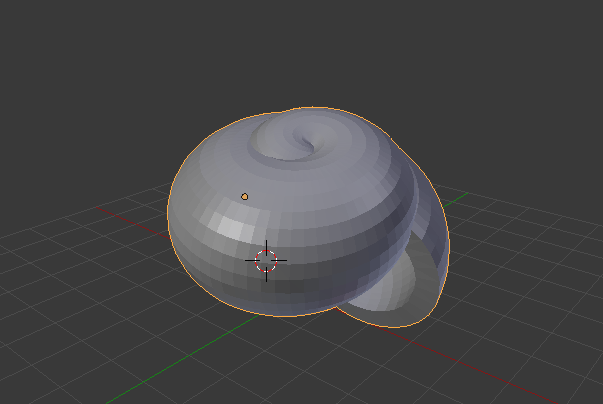
\includegraphics[scale=1.7]{./img/modified_torus_blender.png}
	\caption{Solidified XYZ Math Surface in blender. Exported as \textit{modified\_torus.stl}.
	}
	\label{blender-modified-torus} % Unique label used for referencing the figure in-text
	%\addcontentsline{toc}{figure}{Figure \ref{fig:placeholder}} % Uncomment to add the figure to the table of contents
\end{figure}

\pagebreak

Then it was 3-D printed.

\begin{figure}[h]
	\centering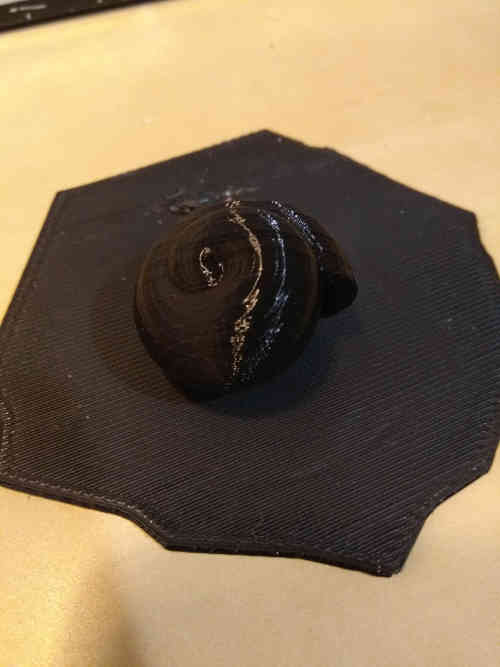
\includegraphics[scale=0.5]{./img/printed_modified_torus.jpg}
	\caption{Printed from \textit{modified\_torus.stl}.}
	\label{3d-printed-torus} % Unique label used for referencing the figure in-text
	%\addcontentsline{toc}{figure}{Figure \ref{fig:placeholder}} % Uncomment to add the figure to the table of contents
\end{figure}

\subsection{Generating Curve} 

Here is a summary of the generating curve method. For a more detailed explanation see \cite{JORGEPICADO}.

\subsubsection{Processing}

\subsubsection{Blender}

\section{Reaction Diffusion Shaders}

In order to model the protrusion of hexaplex radix an RD texture was created. Notice from Figure X that on hexaplex radix the pattern of the protrusions seems to originate from some kind of sinusoidal shape.

\begin{figure}[h]
	\centering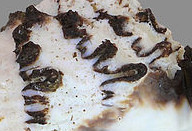
\includegraphics[scale=1.0]{./img/hexaplex_radix_sine.jpg}
	\caption{Sinusoidal pattern on hexaplex radix.}
	\label{hexaplex-sine} % Unique label used for referencing the figure in-text
	%\addcontentsline{toc}{figure}{Figure \ref{fig:placeholder}} % Uncomment to add the figure to the table of contents
\end{figure}

The RD equation used is based on equation 2.4 from \cite{abss}, which uses an activator-inhibitor model.

\begin{equation}
	\frac{\partial a}{\partial t} = \sigma b a^{*2} - r_a a + D_a \frac{\partial^2 a }{\partial x^2}
\end{equation}

\begin{equation}
	\frac{\partial b}{\partial t} = b_b - \sigma b a^{*2} + D_b \frac{\partial^2 b }{\partial x^2}
\end{equation}

\begin{equation*}
	a^{*2} = \frac{a^2}{1+s_a a^2} + b_a
\end{equation*}

\begin{equation*}
\sigma = \rho + r_a  [\tau + \nu \sum_{i=1}^{\eta}{sin(x \cdot rand())}]
\end{equation*}

$a$ represents the concentration of activator and $b$ represents the concentration of inhibitor. $\sigma b a^{*2}$ is the production rate for $a$, and $b_b$ is the production rate for $b$. $-r_a a$ is the depletion of $a$, and $-\sigma b a^{*2}$ is the depletion rate for $b$. $D_a \frac{\partial^2 a }{\partial x^2}$ is the exchange by diffusion. $\sigma$ is mainly a superposition of $sin$ waves to give the pattern a chaotic appearance. This produces a 1-D cellular automata, where the x-axis represents the position and the y-axis represents time.

\begin{figure}[h]
	\centering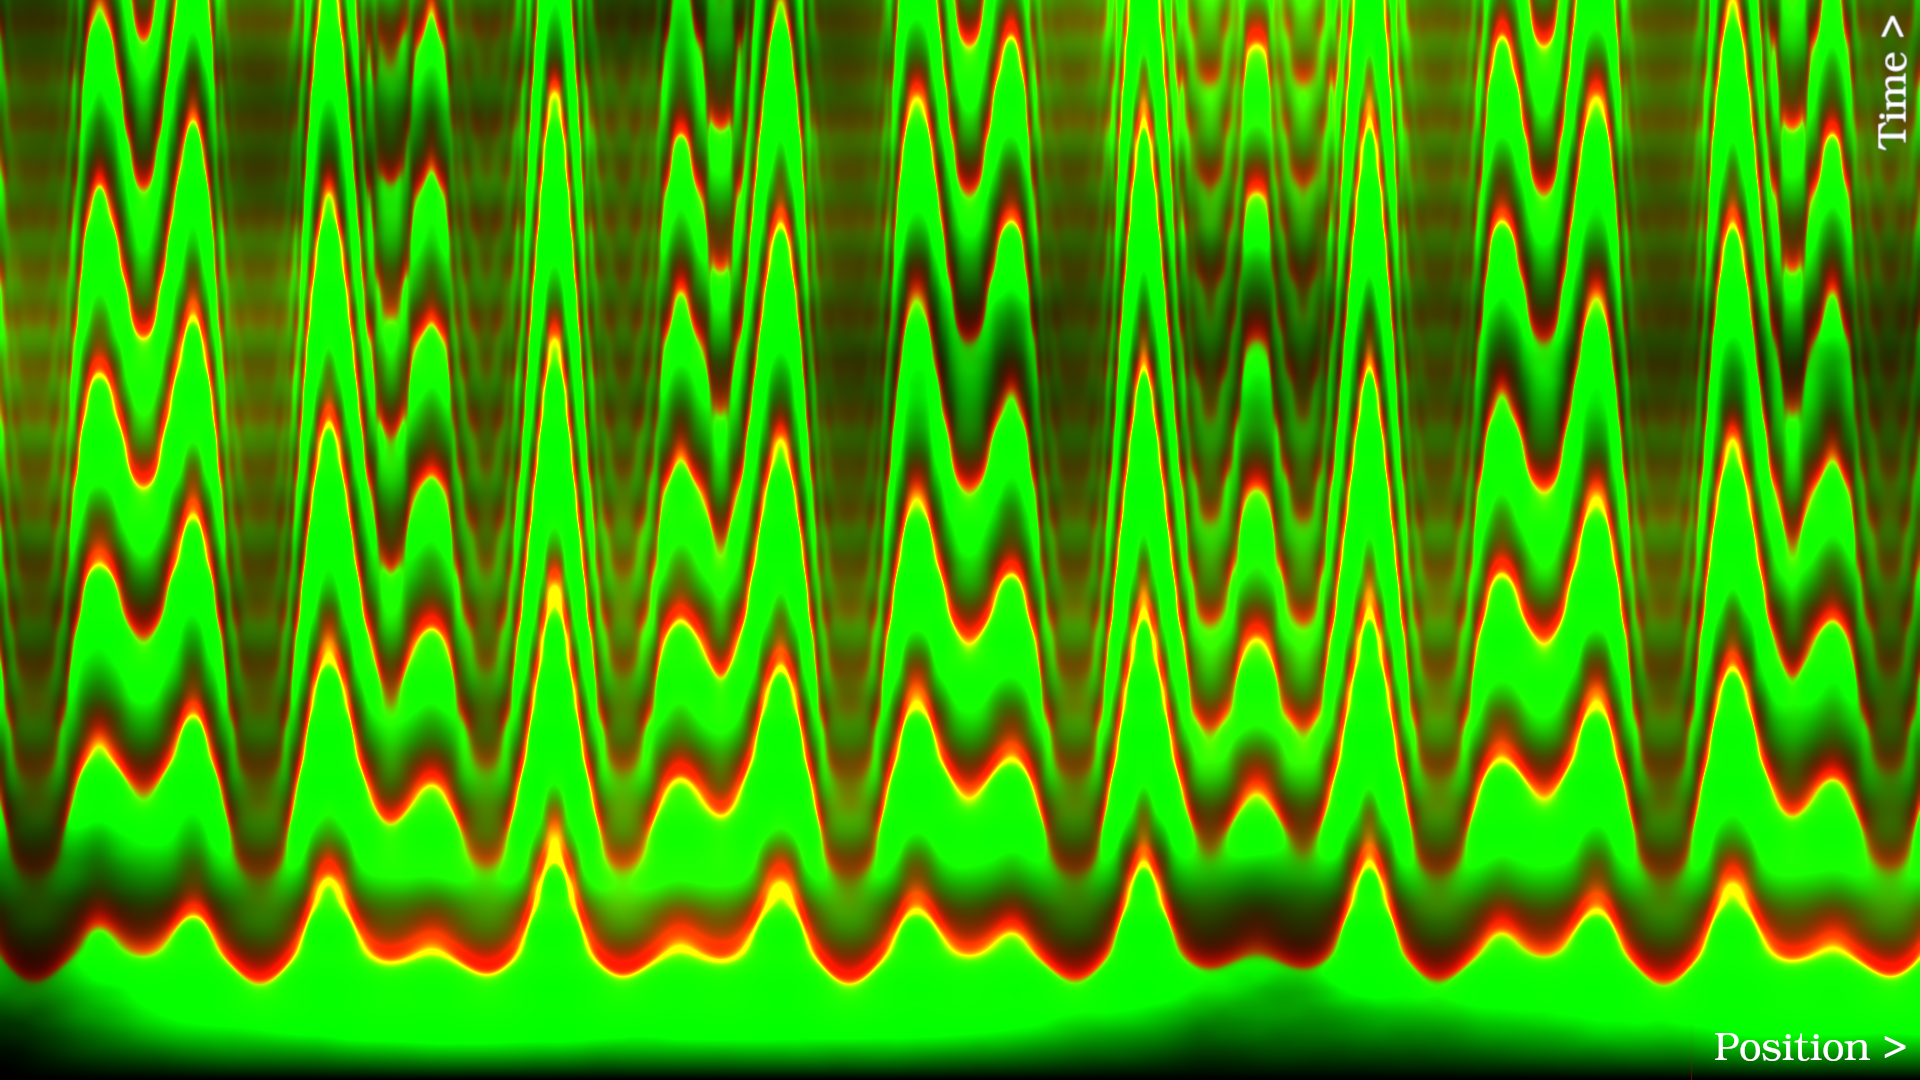
\includegraphics[scale=0.8]{./img/meinhardt-hexaplex-activator-inhibitor.png}
	\caption{Image created from equations (7) and (8). Green value is inhibitor, red is activator. Each value is multiplied by the Fractal Brownian Motion shader. \cite{rd-fbm}}
	\label{activator-inhibitor} % Unique label used for referencing the figure in-text
	%\addcontentsline{toc}{figure}{Figure \ref{fig:placeholder}} % Uncomment to add the figure to the table of contents
\end{figure}

Because the protrusion of hexaplex radix have a mountainous appearance, it seemed appropriate to try adding some fractal noise the final image. An addition shader was created which multiplies the values of the activator-inhibitor shader by fractal brownian motion (FBM) described in \cite{fbm}. It is difficult to notice in Figure X, because the RGB values are not clamp to 0 to 1 in the RD shader. Perhaps this should be changed in later attempts.

\begin{figure}[h]
\centering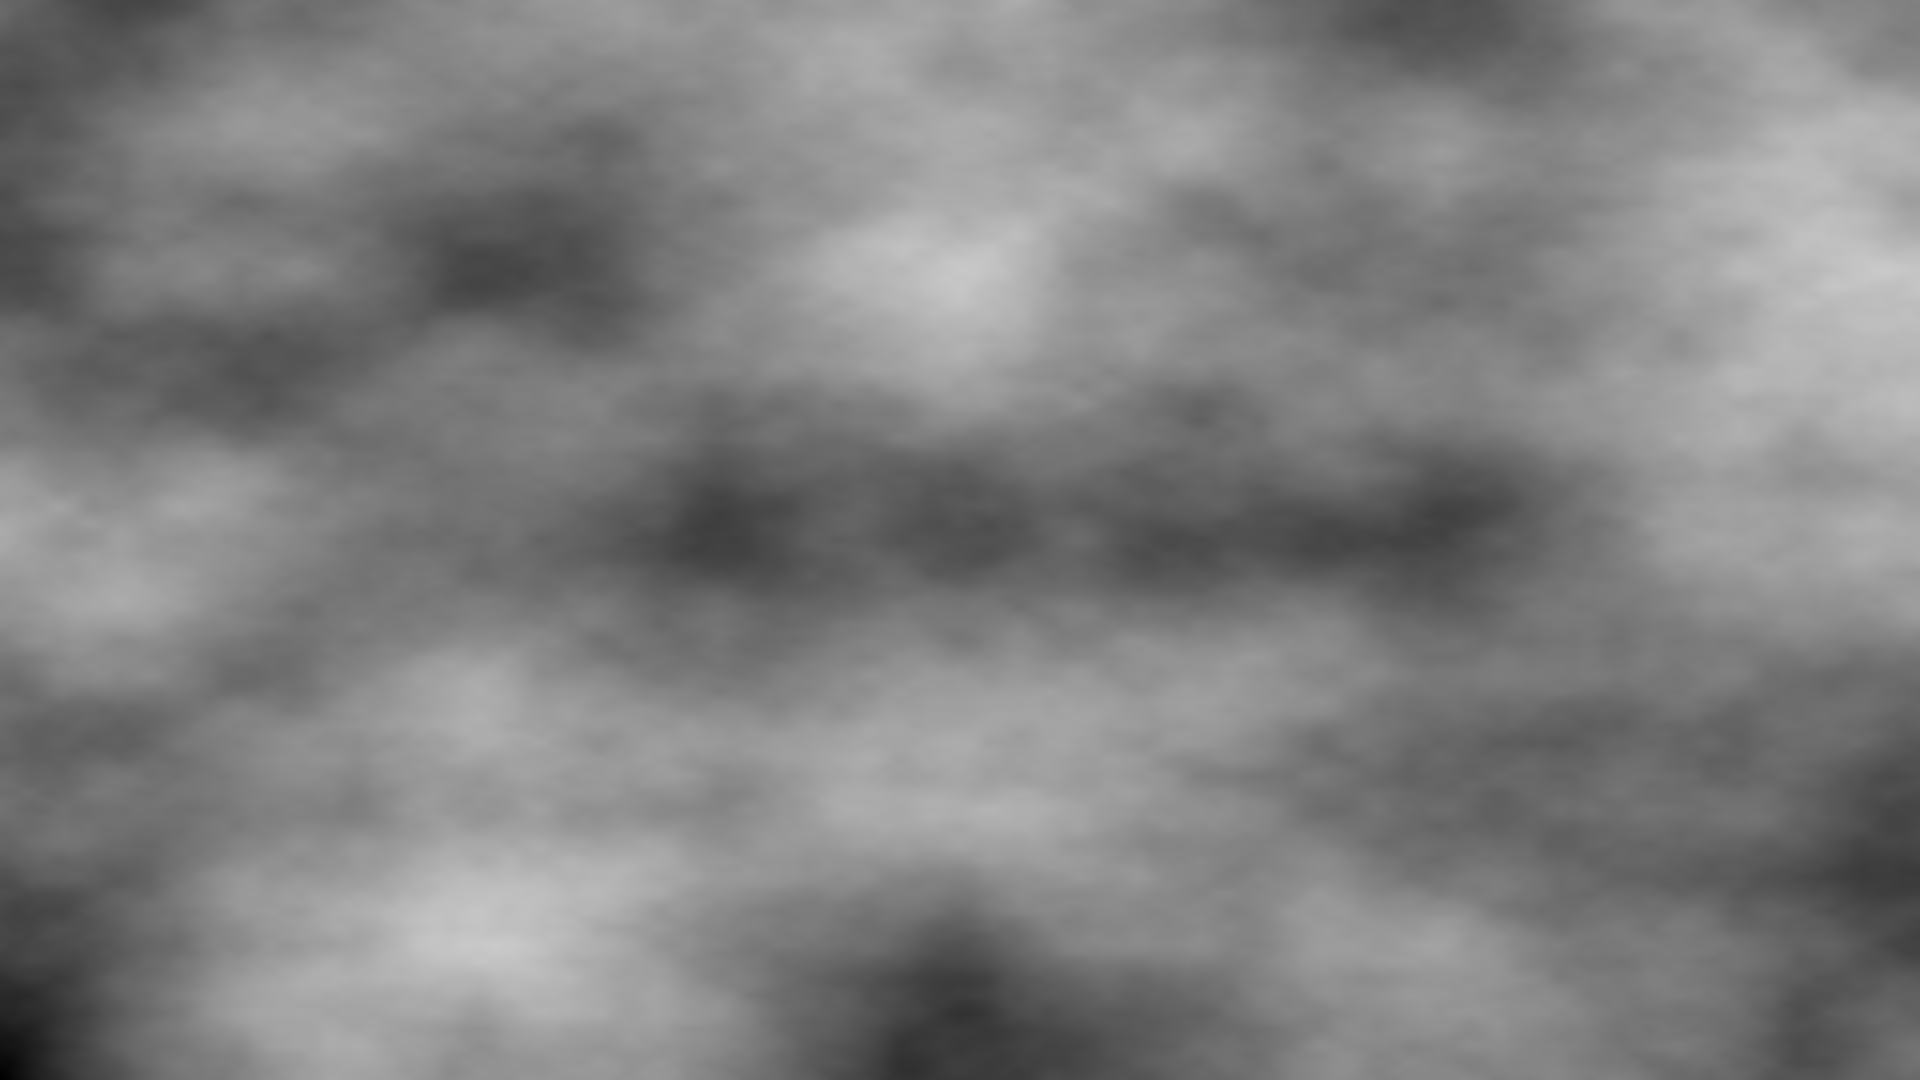
\includegraphics[scale=0.2]{./img/fbm.png}
\caption{Fractal Brownian motion. \cite{st-fbm}}
\label{fbm} % Unique label used for referencing the figure in-text
%\addcontentsline{toc}{figure}{Figure \ref{fig:placeholder}} % Uncomment to add the figure to the table of contents
\end{figure}



\begin{figure}[h]
	\centering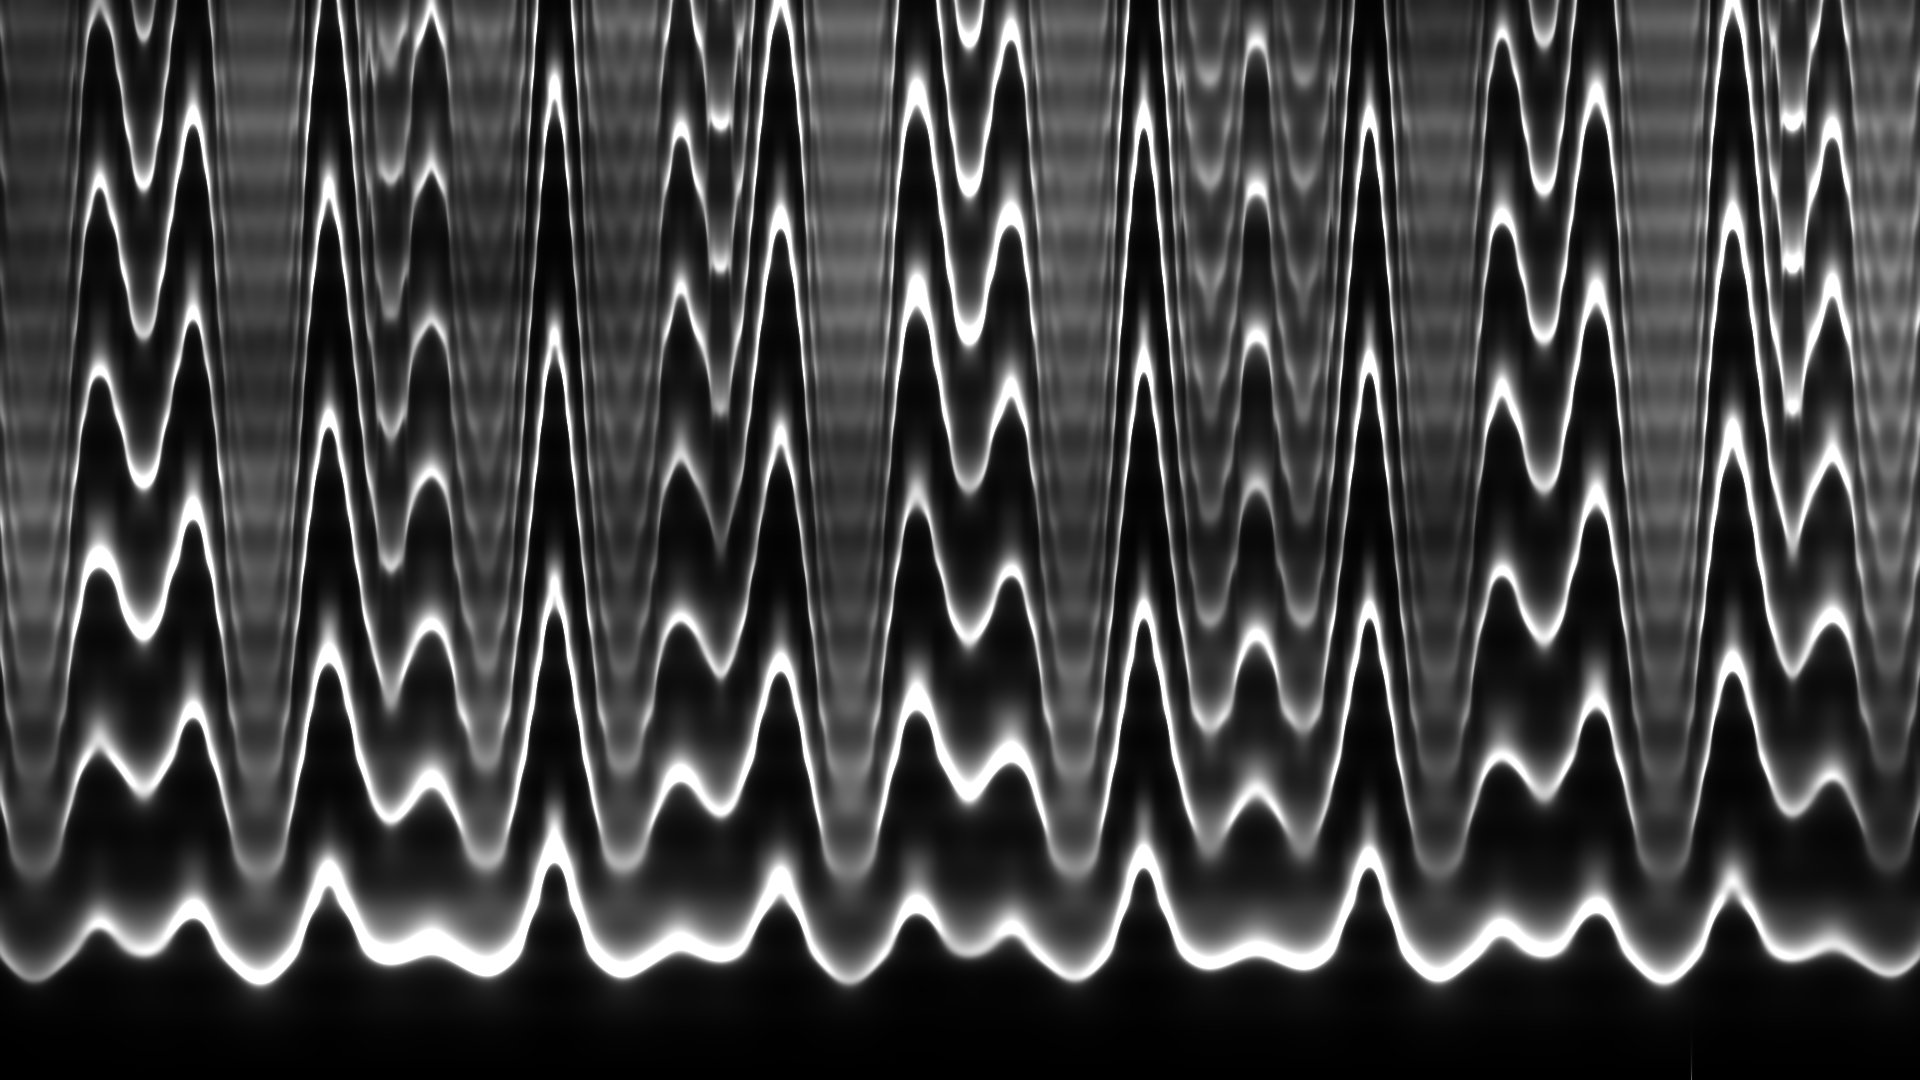
\includegraphics[scale=0.2]{./img/meinhardt-hexaplex.png}
	\caption{Actual height map texture. Red activator value becomes the white color. }
	\label{activator} % Unique label used for referencing the figure in-text
	%\addcontentsline{toc}{figure}{Figure \ref{fig:placeholder}} % Uncomment to add the figure to the table of contents
\end{figure}


\section{Conclusion}

Here is the final model in Blender:

\begin{figure}[h]
	\centering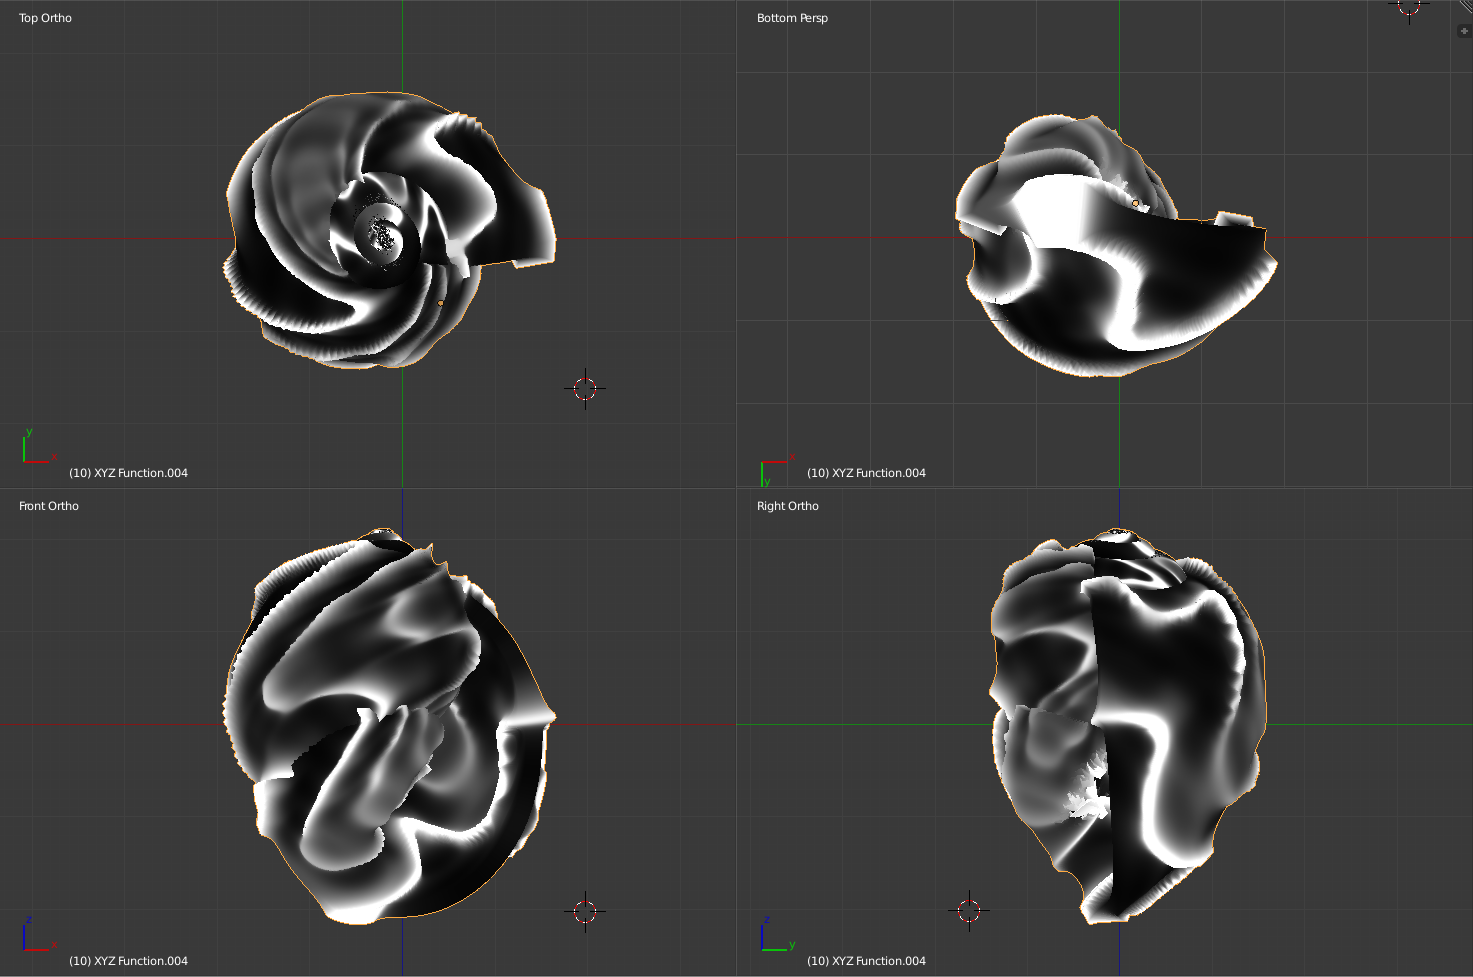
\includegraphics[scale=1.0]{./img/hexaplex_quad.png}
	\caption{Printed from \textit{modified\_torus.stl}.}
	\label{3d-printed-torus} % Unique label used for referencing the figure in-text
	%\addcontentsline{toc}{figure}{Figure \ref{fig:placeholder}} % Uncomment to add the figure to the table of contents
\end{figure}

The UV mapping onto the texture:

\begin{figure}[h]
	\centering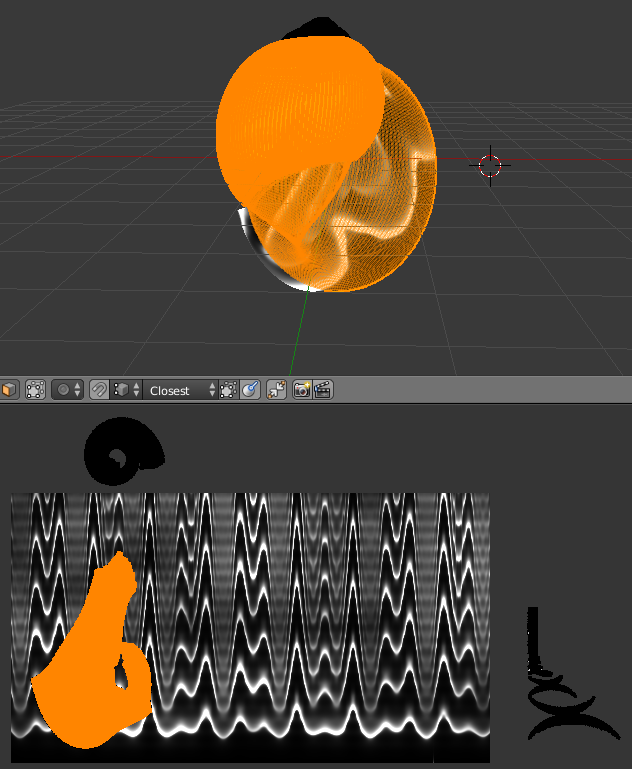
\includegraphics[scale=1.25]{./img/uv_map.png}
	\caption{Printed from \textit{modified\_torus.stl}.}
	\label{3d-printed-torus} % Unique label used for referencing the figure in-text
	%\addcontentsline{toc}{figure}{Figure \ref{fig:placeholder}} % Uncomment to add the figure to the table of contents
\end{figure}

I think it looks better with height map inverted.

\begin{figure}[h]
	\centering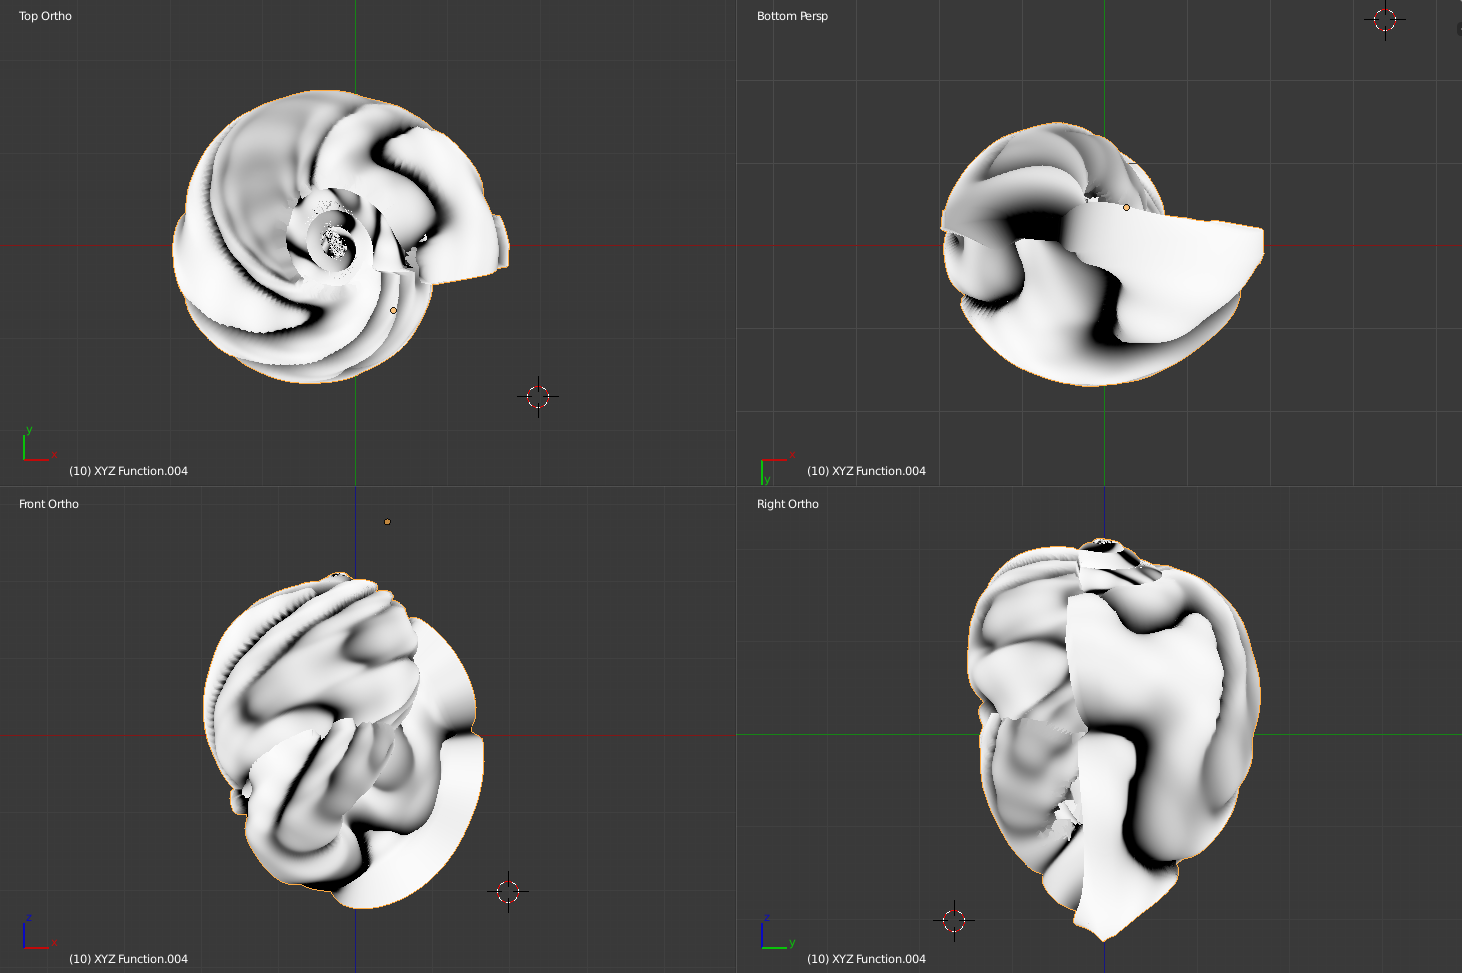
\includegraphics[scale=1.0]{./img/hexaplex_quad_inverted.png}
	\caption{Printed from \textit{modified\_torus.stl}.}
	\label{3d-printed-torus} % Unique label used for referencing the figure in-text
	%\addcontentsline{toc}{figure}{Figure \ref{fig:placeholder}} % Uncomment to add the figure to the table of contents
\end{figure}

\subsection{Future Work}



\bibliographystyle{plain}
\bibliography{refs}

\end{document}